\begin{figure}[htbp]
\section*{ CLDN16}
\centering
\begin{subfigure}[b]{0.95\textwidth}
\centering
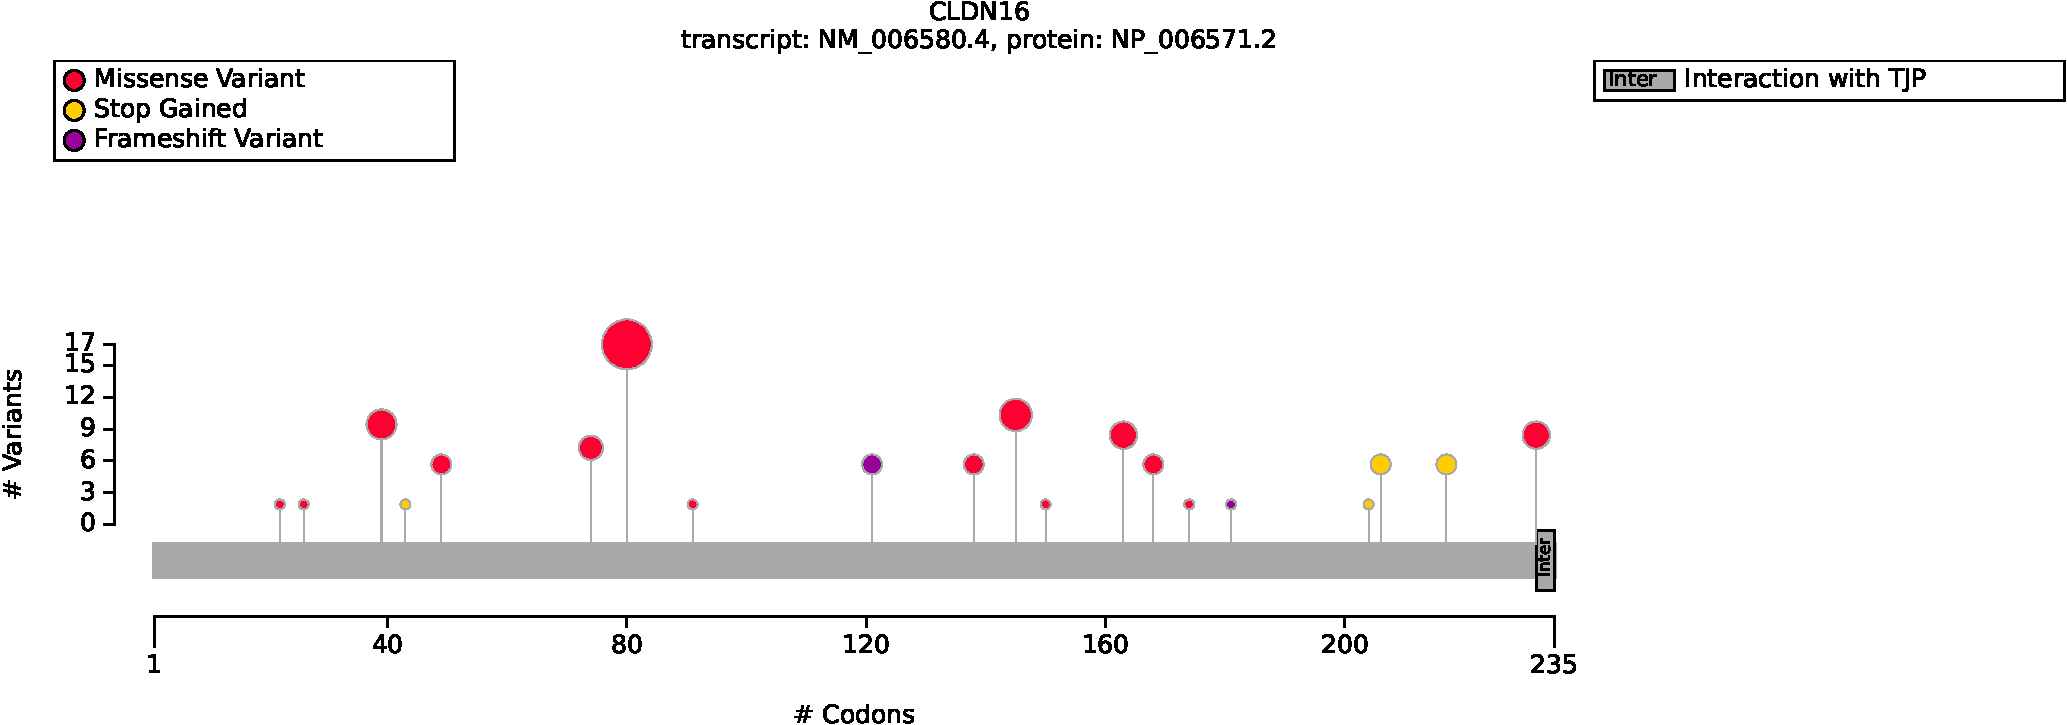
\includegraphics[width=\textwidth]{ img/CLDN16_protein_diagram.pdf} 
\captionsetup{justification=raggedright,singlelinecheck=false}
\caption{Distribution of variants in CLDN16}
\end{subfigure}

\vspace{2em}

\begin{subfigure}[b]{0.95\textwidth}
\centering
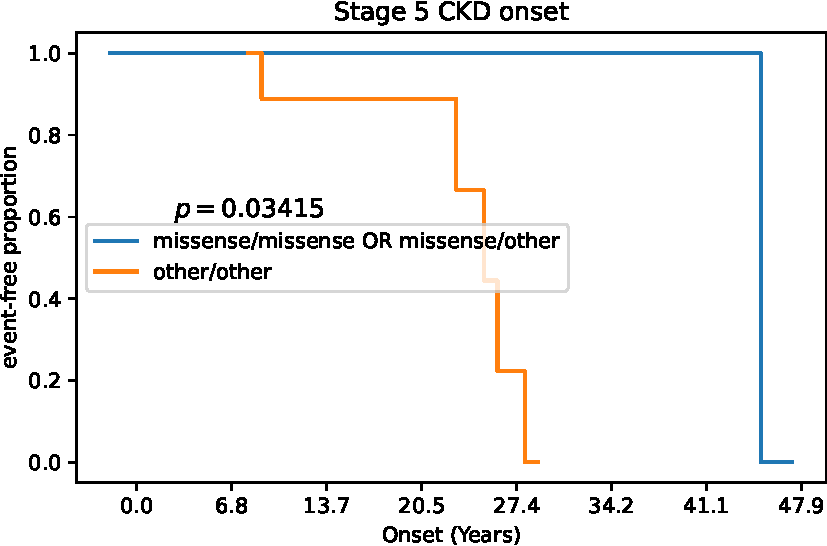
\includegraphics[width=0.3\textwidth]{ img/CLDN16_stats.pdf} 
\captionsetup{justification=raggedright,singlelinecheck=false}
\caption{Onset of stage 5 chronic kidney disease for CLDN16 missense vs. other variants. This result is similar to that of Konrad et al. (2008) \cite{PMID_18003771}.}
\end{subfigure}

\vspace{2em}

\begin{subfigure}[b]{0.95\textwidth}
\centering
\resizebox{\textwidth}{!}{
\begin{tabular}{llllrr}
\toprule
Genotype (A) & Genotype (B) & total tests performed & significant results\\
\midrule
Leu81Phe/Leu81Phe & other/other OR Leu81Phe/other & 26 & 0\\
missense/missense OR missense/other & other/other & 23 & 0\\
FEMALE & MALE & 27 & 0\\
\bottomrule
\end{tabular}
}
\captionsetup{justification=raggedright,singlelinecheck=false}
\caption{Fisher Exact Test performed to compare HPO annotation frequency with respect to genotypes.}
\end{subfigure}

\vspace{2em}

\begin{subfigure}[b]{0.95\textwidth}
\captionsetup{justification=raggedright,singlelinecheck=false}
\resizebox{\textwidth}{!}{
\begin{tabular}{llllrr}
\toprule
Description & Variable & Genotype (A) & Genotype (B) & p-value & xrefs\\
\midrule
Hypomagnesemia 3, renal (OMIM:248250) disease onset & Onset of OMIM:248250 & missense/missense OR missense/other & other/other & 0.333 & \cite{PMID_18003771}\\
\bottomrule
\end{tabular}
}
\caption{ Onset of OMIM:248250 to compare missense/missense OR missense/other and other/other with respect to Onset of OMIM:248250. }
\end{subfigure}

\vspace{2em}

\begin{subfigure}[b]{0.95\textwidth}
\captionsetup{justification=raggedright,singlelinecheck=false}
\resizebox{\textwidth}{!}{
\begin{tabular}{llllrr}
\toprule
Description & Variable & Genotype (A) & Genotype (B) & p-value & xrefs\\
\midrule
Survival analysis: Stage 5 chronic kidney disease & Onset of HP:0003774 & missense/missense OR missense/other & other/other & 0.034 & \cite{PMID_18003771}\\
\bottomrule
\end{tabular}
}
\caption{Onset of Stage 5 chronic kidney disease to compare missense/missense OR missense/other and other/other with respect to Onset of HP:0003774. }
\end{subfigure}

\vspace{2em}

\caption{ The cohort comprised 51 individuals (21 females, 29 males, 1 with unknown sex). A total of 53 HPO terms were used to annotate the cohort. Disease diagnosis: Hypomagnesemia 3, renal (OMIM:248250). to do. A total of 23 unique variant alleles were found in \textit{CLDN16} (transcript: \texttt{NM\_006580.4}, protein id: \texttt{NP\_006571.2}).}
\end{figure}
